\documentclass[ucs,9pt]{beamer}

% Copyright 2004 by Till Tantau <tantau@users.sourceforge.net>.
%
% In principle, this file can be redistributed and/or modified under
% the terms of the GNU Public License, version 2.
%
% However, this file is supposed to be a template to be modified
% for your own needs. For this reason, if you use this file as a
% template and not specifically distribute it as part of a another
% package/program, I grant the extra permission to freely copy and
% modify this file as you see fit and even to delete this copyright
% notice.
%
% Modified by Tobias G. Pfeiffer <tobias.pfeiffer@math.fu-berlin.de>
% to show usage of some features specific to the FU Berlin template.

% remove this line and the "ucs" option to the documentclass when your editor is not utf8-capable
\usepackage[utf8x]{inputenc}    % to make utf-8 input possible
\usepackage[english]{babel}     % hyphenation etc., alternatively use 'german' as parameter

% Template for talks using the Corporate Design of the Freie Universitaet
%   Berlin, created following the guidelines on www.fu-berlin.de/cd by
%   Tobias G. Pfeiffer, <tobias.pfeiffer@math.fu-berlin.de>
% This file can be redistributed and/or modified in any way you like.
%   If you feel you have done significant improvements to this template,
%   please consider providing your modified version to
%   https://www.mi.fu-berlin.de/w/Mi/BeamerTemplateCorporateDesign

\usepackage{amsmath,dsfont,listings}

%%% FU logo
% small version for upper right corner of normal pages
\pgfdeclareimage[height=0.9cm]{university-logo}{FULogo_RGB}
\logo{\pgfuseimage{university-logo}}
% large version for upper right corner of title page
\pgfdeclareimage[height=1.085cm]{big-university-logo}{FULogo_RGB}
\newcommand{\titleimage}[1]{\pgfdeclareimage[height=2.92cm]{title-image}{#1}}
\titlegraphic{\pgfuseimage{title-image}}
%%% end FU logo

% NOTE: 1cm = 0.393 in = 28.346 pt;    1 pt = 1/72 in = 0.0352 cm
\setbeamersize{text margin right=3.5mm, text margin left=7.5mm}  % text margin

% colors to be used
\definecolor{text-grey}{rgb}{0.45, 0.45, 0.45} % grey text on white background
\definecolor{bg-grey}{rgb}{0.66, 0.65, 0.60} % grey background (for white text)
\definecolor{fu-blue}{RGB}{0, 51, 102} % blue text
\definecolor{fu-green}{RGB}{153, 204, 0} % green text
\definecolor{fu-red}{RGB}{204, 0, 0} % red text (used by \alert)

% switch off the sidebars
% TODO: loading \useoutertheme{sidebar} (which is maybe wanted) also inserts
%   a sidebar on title page (unwanted), also indents the page title (unwanted?),
%   and duplicates the navigation symbols (unwanted)
\setbeamersize{sidebar width left=0cm, sidebar width right=0mm}
\setbeamertemplate{sidebar right}{}
\setbeamertemplate{sidebar left}{}
%    XOR
% \useoutertheme{sidebar}

% frame title
% is truncated before logo and splits on two lines
% if neccessary (or manually using \\)
\setbeamertemplate{frametitle}{%
    \vskip-30pt \color{text-grey}\large%
    \begin{minipage}[b][23pt]{80.5mm}%
    \flushleft\insertframetitle%
    \end{minipage}%
}

%%% title page
% TODO: get rid of the navigation symbols on the title page.
%   actually, \frame[plain] *should* remove them...
\setbeamertemplate{title page}{
% upper right: FU logo
\vskip2pt\hfill\pgfuseimage{big-university-logo} \\
\vskip6pt\hskip3pt
% title image of the presentation
\begin{minipage}{11.6cm}
\hspace{-1mm}\inserttitlegraphic
\end{minipage}

% set the title and the author
\vskip14pt
\parbox[top][1.35cm][c]{11cm}{\color{text-grey}\inserttitle \\ \small \insertsubtitle}
\vskip11pt
\parbox[top][1.35cm][c]{11cm}{\small \insertauthor \\ \insertinstitute \\[3mm] \insertdate}
}
%%% end title page

%%% colors
\usecolortheme{lily}
\setbeamercolor*{normal text}{fg=black,bg=white}
\setbeamercolor*{alerted text}{fg=fu-red}
\setbeamercolor*{example text}{fg=fu-green}
\setbeamercolor*{structure}{fg=fu-blue}

\setbeamercolor*{block title}{fg=white,bg=black!50}
\setbeamercolor*{block title alerted}{fg=white,bg=black!50}
\setbeamercolor*{block title example}{fg=white,bg=black!50}

\setbeamercolor*{block body}{bg=black!10}
\setbeamercolor*{block body alerted}{bg=black!10}
\setbeamercolor*{block body example}{bg=black!10}

\setbeamercolor{bibliography entry author}{fg=fu-blue}
% TODO: this doesn't work at all:
\setbeamercolor{bibliography entry journal}{fg=text-grey}

\setbeamercolor{item}{fg=fu-blue}
\setbeamercolor{navigation symbols}{fg=text-grey,bg=bg-grey}
%%% end colors

%%% headline
\setbeamertemplate{headline}{
\vskip4pt\hfill\insertlogo\hspace{3.5mm} % logo on the right

\vskip6pt\color{fu-blue}\rule{\textwidth}{0.4pt} % horizontal line
}
%%% end headline

%%% footline
\newcommand{\footlinetext}{\insertshortinstitute, \insertshorttitle, \insertshortdate}
\setbeamertemplate{footline}{
\vskip5pt\color{fu-blue}\rule{\textwidth}{0.4pt}\\ % horizontal line
\vskip2pt
\makebox[123mm]{\hspace{7.5mm}
\color{fu-blue}\footlinetext
\hfill \raisebox{-1pt}{\usebeamertemplate***{navigation symbols}}
\hfill \insertframenumber}
\vskip4pt
}
%%% end footline

%%% settings for listings package
\lstset{extendedchars=true, showstringspaces=false, basicstyle=\footnotesize\sffamily, tabsize=2, breaklines=true, breakindent=10pt, frame=l, columns=fullflexible}
\lstset{language=Java} % this sets the syntax highlighting
\lstset{mathescape=true} % this switches on $...$ substitution in code
% enables UTF-8 in source code:
\lstset{literate={ä}{{\"a}}1 {ö}{{\"o}}1 {ü}{{\"u}}1 {Ä}{{\"A}}1 {Ö}{{\"O}}1 {Ü}{{\"U}}1 {ß}{\ss}1}
%%% end listings  % THIS is the line that includes the FU template!

\usepackage{arev,t1enc} % looks nicer than the standard sans-serif font
% if you experience problems, comment out the line above and change
% the documentclass option "9pt" to "10pt"

% image to be shown on the title page (without file extension, should be pdf or png)
\titleimage{fu_500}

\title[BGP Data] % (optional, use only with long paper titles)
{Processing of Live BGP Data with BGPStream}

%\subtitle
%{Include Only If Paper Has a Subtitle}

\author[Author, Another] % (optional, use only with lots of authors)
{A.~Kurth \and Y.~Lewash \and S. Sontberg}
% - Give the names in the same order as the appear in the paper.

\institute[FU Berlin] % (optional, but mostly needed)
{Freie Universität Berlin}
% - Keep it simple, no one is interested in your street address.

\date[SWP 2017] % (optional, should be abbreviation of conference name)
{Softwareprojekt Internetkommunikation, 2017}
% - Either use conference name or its abbreviation.
% - Not really informative to the audience, more for people (including
%   yourself) who are reading the slides online

\subject{Technische Informatik}
% This is only inserted into the PDF information catalog. Can be left
% out.

% you can redefine the text shown in the footline. use a combination of
% \insertshortauthor, \insertshortinstitute, \insertshorttitle, \insertshortdate, ...
\renewcommand{\footlinetext}{\insertshortinstitute, \insertshorttitle, \insertshortdate}

% Delete this, if you do not want the table of contents to pop up at
% the beginning of each subsection:
%\AtBeginSubsection[]
%{
%  \begin{frame}<beamer>{Outline}
%    \tableofcontents[currentsection,currentsubsection]
%  \end{frame}
%}

\begin{document}

\begin{frame}[plain]
  \titlepage
\end{frame}

%\begin{frame}{Outline}
%  \tableofcontents
%  % You might wish to add the option [pausesections]
%\end{frame}

\section{Motivation}

\subsection{Border Gateway Protocol}

\begin{frame}{Border Gateway Protocol}%{Subtitles are optional.}
  % - A title should summarize the slide in an understandable fashion
  %   for anyone how does not follow everything on the slide itself.
  \begin{itemize}
  \item
    %Use \texttt{itemize} a lot.
    IBGP/EBGP are interior/exterior gateway protocols
  \item
    for exchanging routing and reachability information among autonomous systems
    \begin{itemize}
    \item
      obtain subnet reachability information from external AS
    \item
      propagate reachability information to internal routers
    \item
      determine good/consistent routes to subnets
    \end{itemize}
  \item
    current version 4 is used since 1994
  \end{itemize}
  \pause
  \centering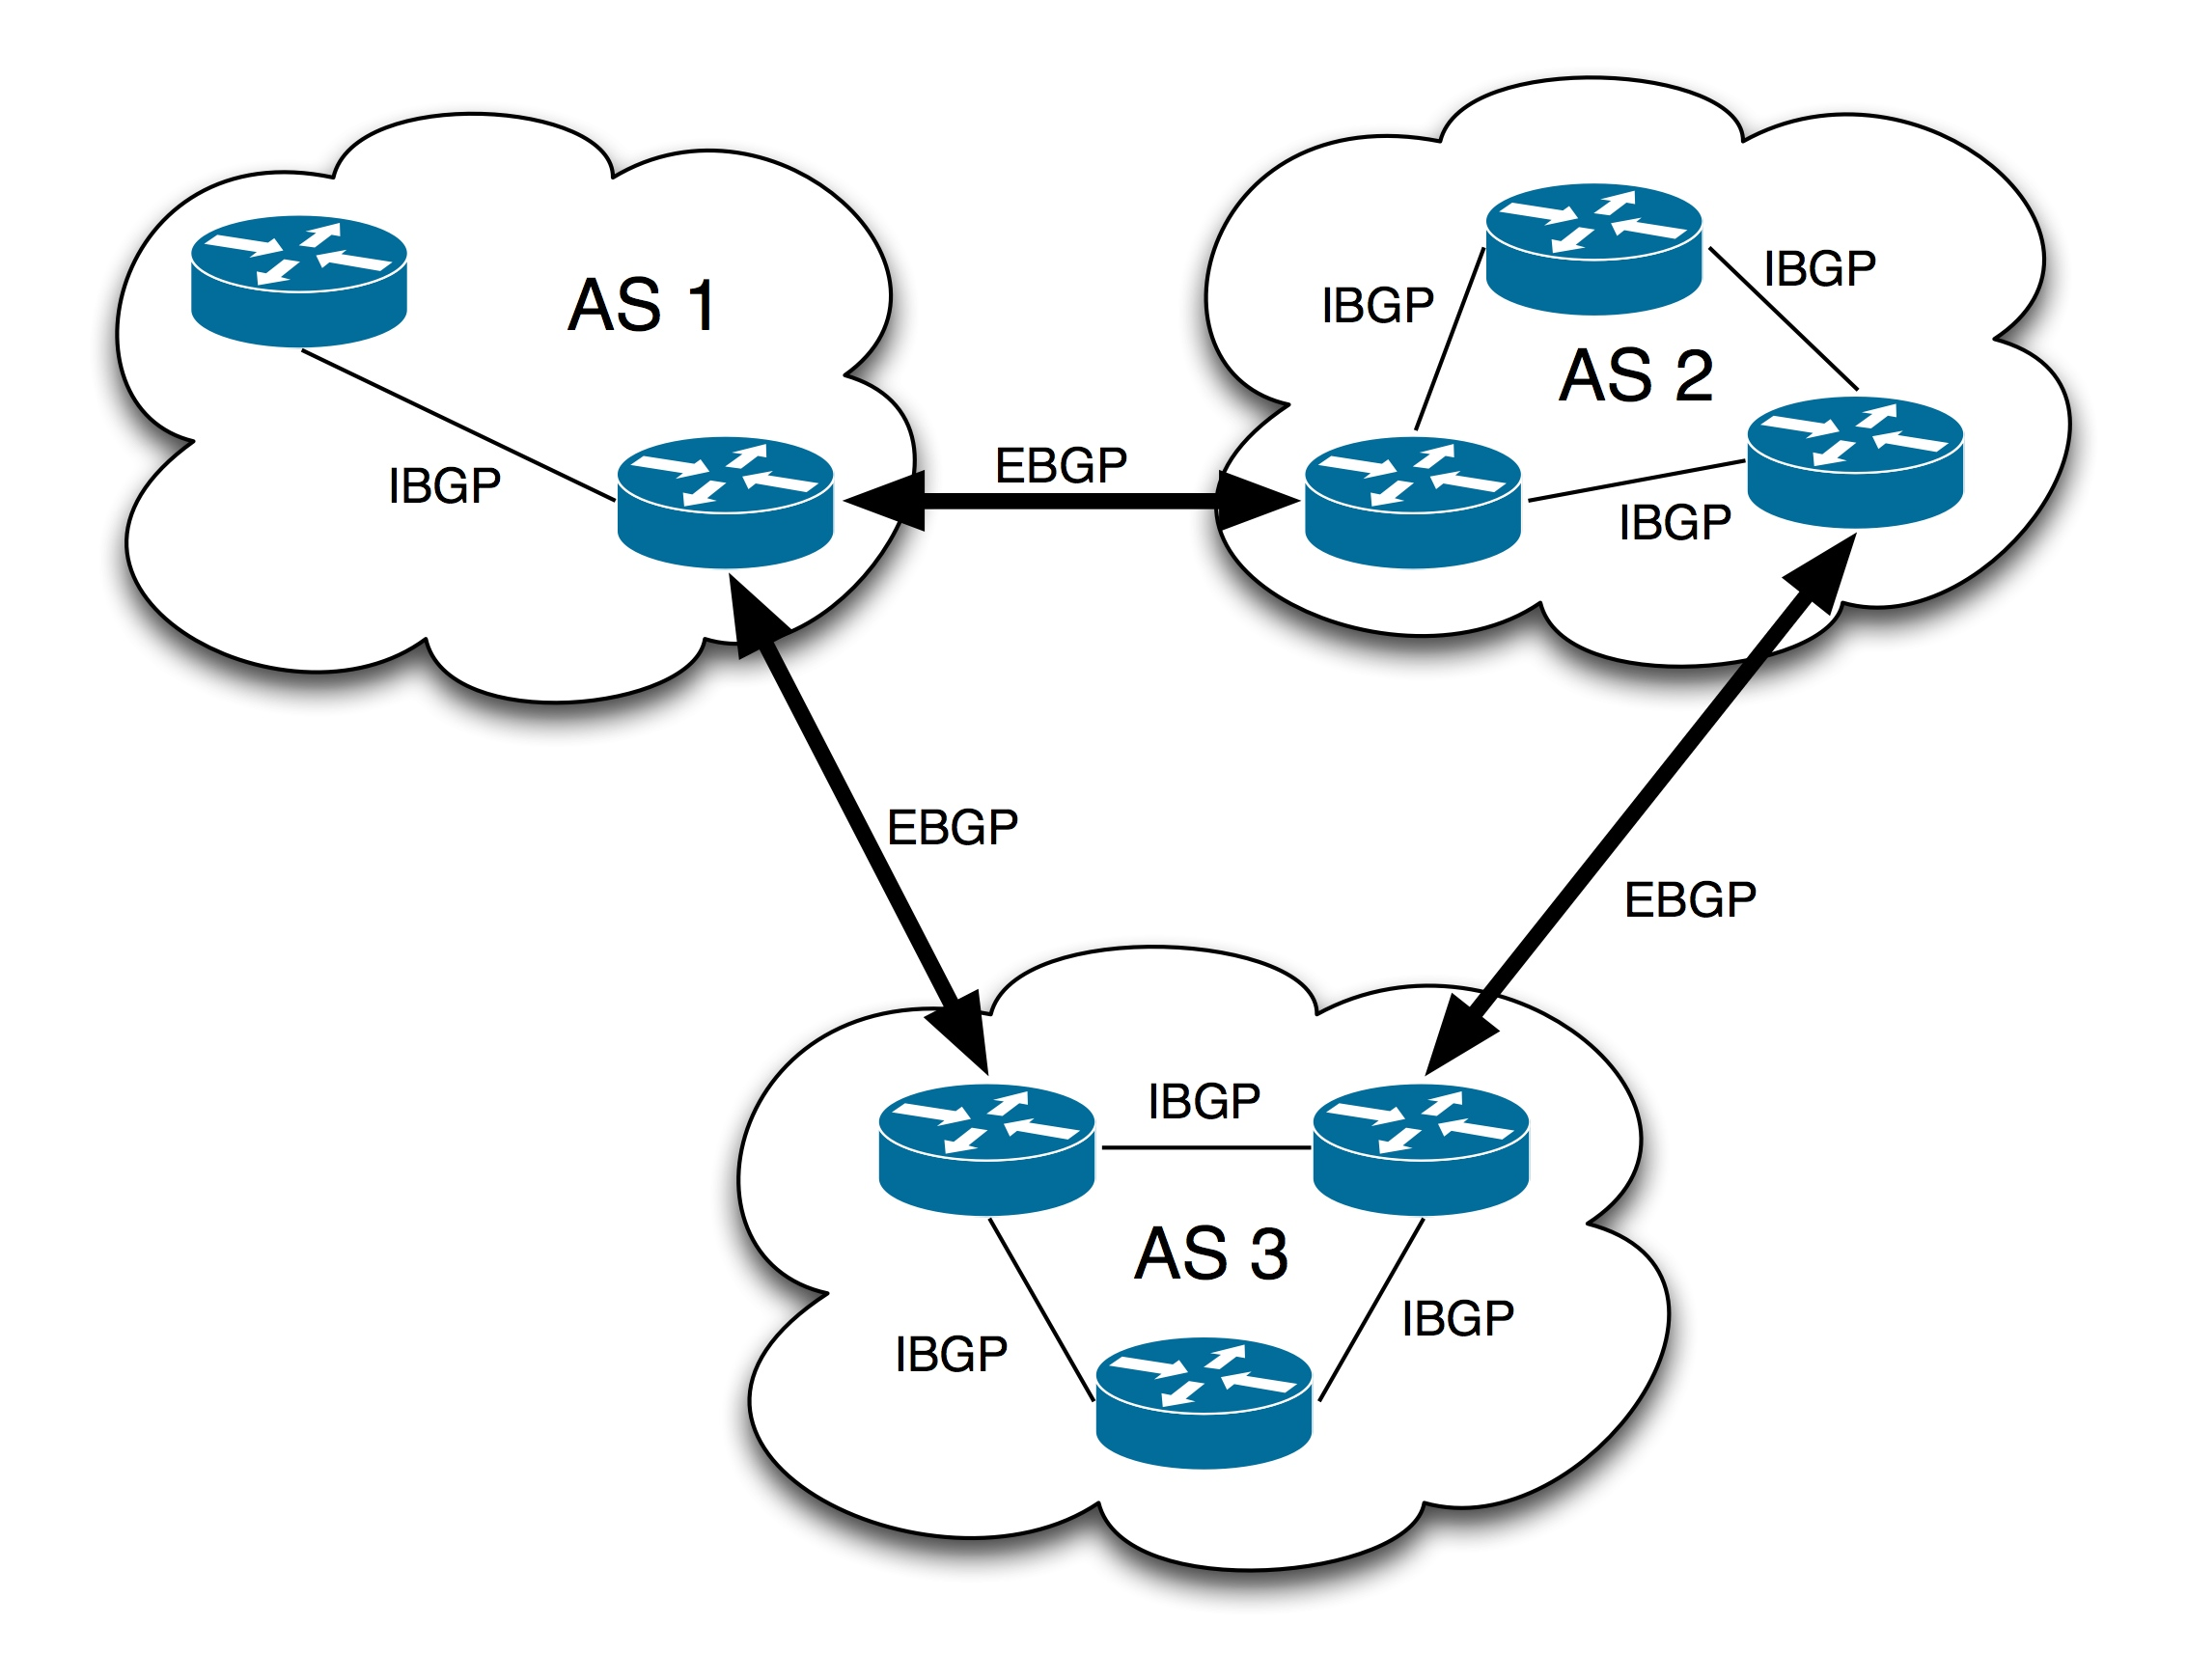
\includegraphics[width=6cm]{bgp}\\
  \tiny{[https://www.noction.com/wp-content/uploads/2012/03/bgp.jpg]}
\end{frame}

\subsection{BGPStream}

\begin{frame}[fragile]{BGPStream}

  %You can create overlays\dots
  \begin{itemize}
  \item
    BGPStream is a framework for live and historical BGP data analysis
    \begin{itemize}
    \item
      APIs for C/C++ and Python
    \item
      can process raw RIS data [http://data.ris.ripe.net/] live
    \end{itemize}
  \item
    e.g. update dumps from RIS RRC00 collector (Amsterdam)\\since May 14, 2017:\\
    % NB. listings is quite powerful, but not well suited to be used with beamer
    %  consider using semiverbatim or the like, see below
    \begin{lstlisting}[language=sh]%[mathescape=false]
      bgpreader -w 1494720000 -c rrc00
      R|R|1494720000|ris|rrc00|22652|45.61.0.85|1.1.251.0/24|45.61.0.85|22652 6453 3491 38040 23969|23969|||
      R|R|1494720000|ris|rrc00|3257|213.200.87.254|1.1.251.0/24|213.200.87.254|3257 3491 38040 23969|23969|3257:8059 3257:30275 3257:50001 3257:54900 3257:54901||
      R|R|1494720000|ris|rrc00|8758|212.25.27.44|1.1.251.0/24|212.25.27.44|8758 8220 38040 23969|23969|8220:65010 8220:65401 8758:110 8758:300||
      R|R|1494720000|ris|rrc00|4608|203.119.76.5|1.1.251.0/24|203.119.76.5|4608 1221 4637 3491 38040 23969|23969|||
      ...
    \end{lstlisting}
  \end{itemize}
\end{frame}

\begin{frame}[fragile]{RTRLib}

  %You can create overlays\dots
  \begin{itemize}
  \item
    A C implementation of the RPKI/Router Protocol client
    \begin{itemize}
    \item
      API for C
    \item
      can verify announcements (IP/prefix <-> ASN) against a RPKI-RTR cache server
    \end{itemize}
  \item
    e.g. IP / prefix length / ASN relation
    \begin{lstlisting}[language=sh]%[mathescape=false]
      + 116.197.131.0                               24 -  24        58369
      + 84.20.48.0                                  21 -  21         6830
      + 31.47.192.0                                 21 -  24        49800
      ...
    \end{lstlisting}
  \end{itemize}
\end{frame}


\section{To do}

\begin{frame}{Our Contribution}

  \begin{itemize}
    \item We need to implement an application to filter, analyze and visualize data according to different parameters.
    \item Implemented in C++
    \item Presentation on console (ncurses, like htop)  
    \item Show coverage of ROAs
    \item Detect BGP prefix hijacking (how often?, how long?)
  \end{itemize}
    
\end{frame}
\end{document}
